\documentclass[12pt]{amsart}   % LaTeX with AMS style; 12 point for old eyes

\usepackage{paper}

\begin{document}

\graphicspath{ {figures/} }

\title[Billiards]{Sequences of Billiard Ball Collisions}

\author{Jonathan Allen, John Wang}
\date{\today}

\maketitle

\subsection*{Abstract}

In this paper we explore properties of sequences of billiard ball collisions. We present a tiling representation which is used to help elucidate some simple properties of these sequences. Then, we provide a one-dimensional representation which builds upon the tiling representation. Next, we provide a method which takes an arbitrary sequence and checks to see if it could have been created by a billiard ball colliding with a billiard table. Finally, we show how these sequences relate to continued fractions.

\section{Introduction}
\frame{
  \frametitle{Introduction}

  \begin{itemize}
    \item Billiard ball bouncing in a square
    \item Assume no gravity or friction
    \item Examine sequence of sides
  \end{itemize}
}

\subsection{Examples}

\frame{
  \frametitle{Example}

  \begin{example}
    Examine the sequence: `abab`
  \end{example}

  \begin{figure}
    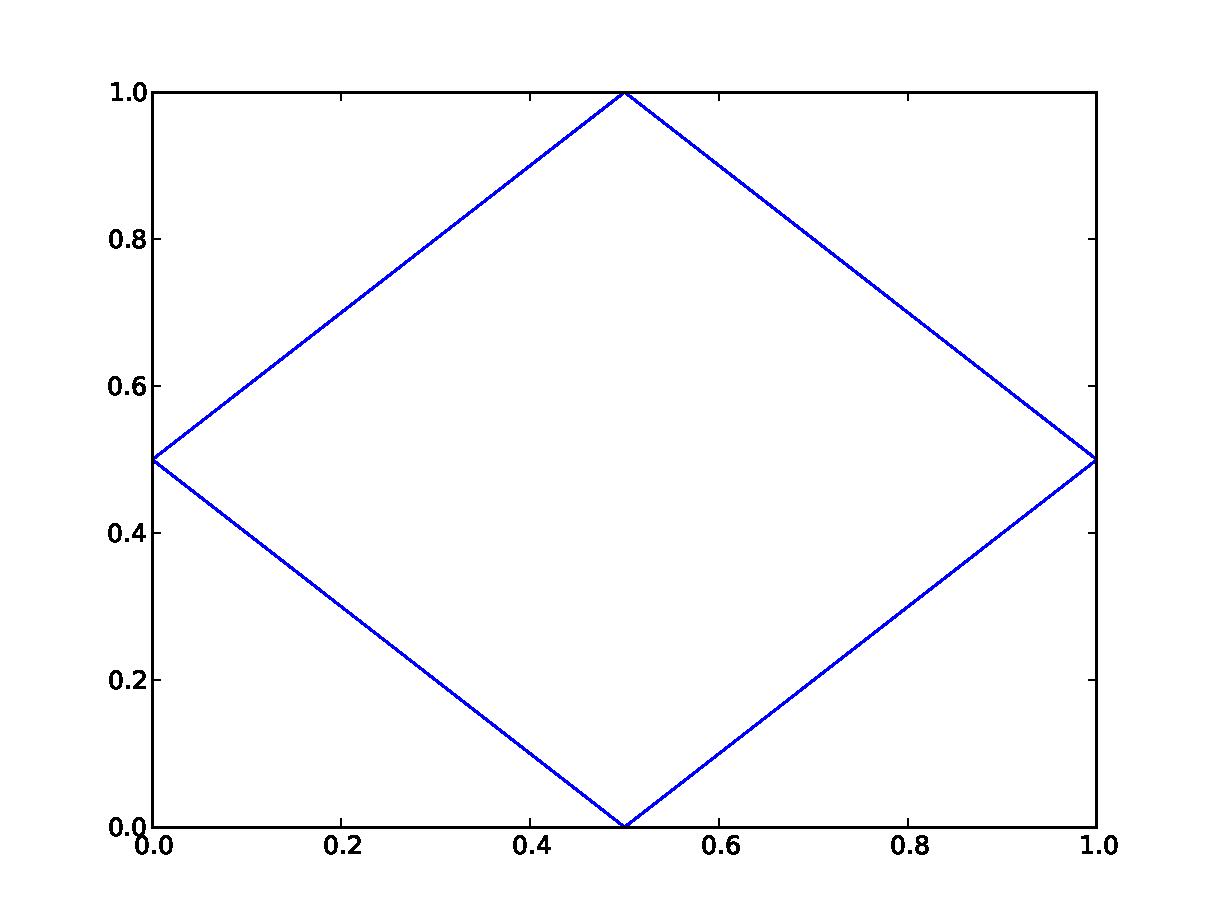
\includegraphics[width=3in]{figures/abab.pdf}
  \end{figure}
}

\frame{
  \frametitle{Another Example}

  \begin{example}
    Examine the sequence: `aaabaaab`
  \end{example}

  \begin{figure}
    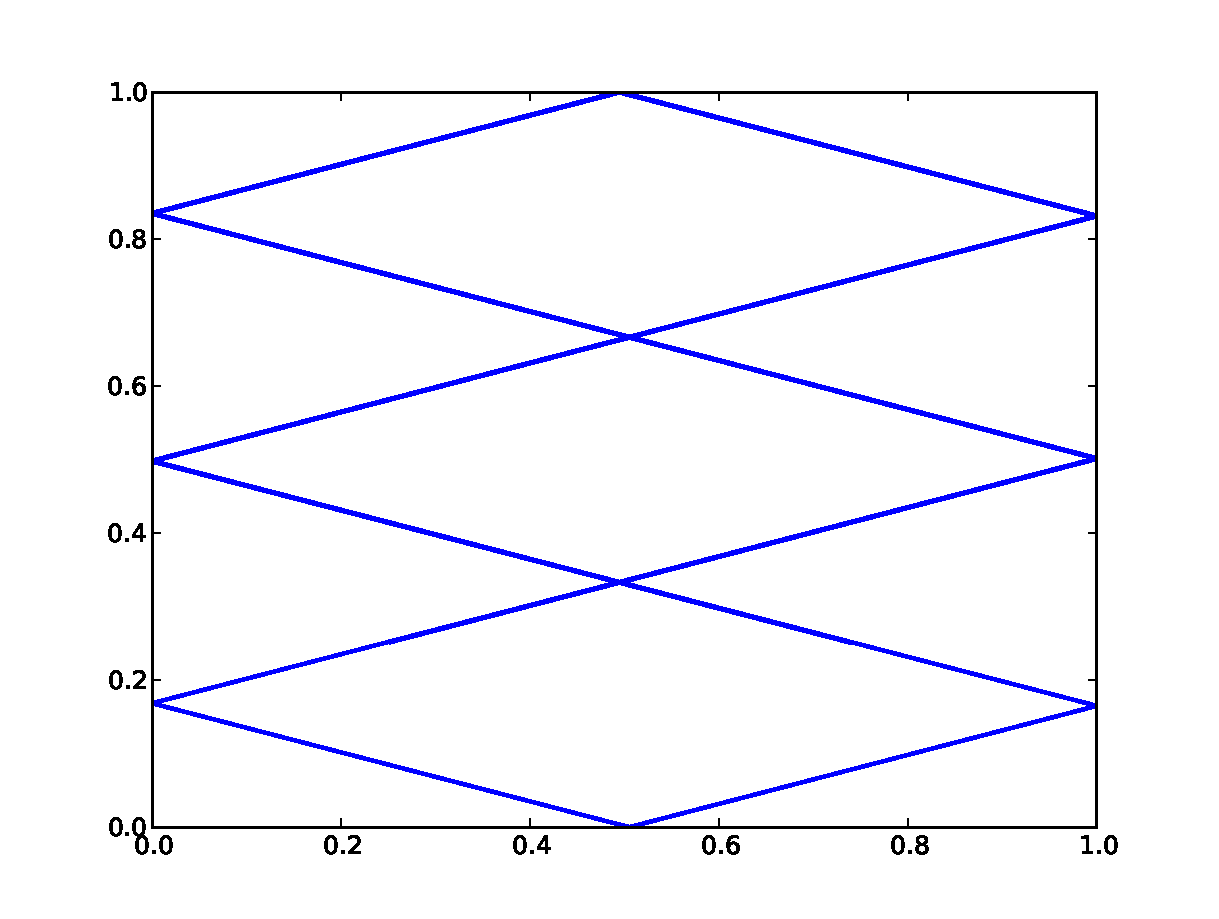
\includegraphics[width=3in]{figures/aaabaaab.pdf}
  \end{figure}
}

\subsection{Outline}

\frame{
  \frametitle{Presentation Outline}
  \tableofcontents
}

\frame{
  \frametitle{Notation}

  \begin{definition}
    A table $T$ is the unit square in $\mathrm{R}^2$. A particle $p \in T$ begins at position $\bar{x}_0 \in T$ with velocity $\bar{v}$. When the particle reaches an edge of the table, velocity is reflected about the line perpendicular to the table's edge.
  \end{definition}

  \begin{figure}
    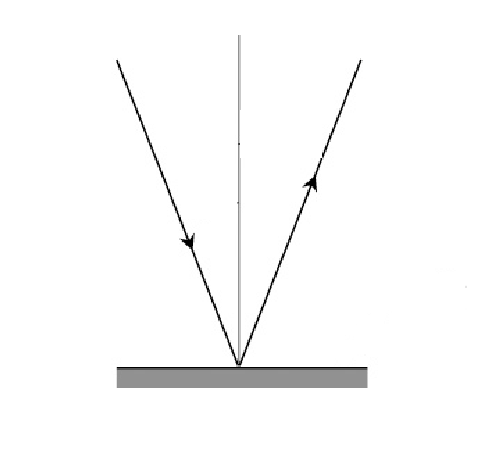
\includegraphics[width=2in]{figures/particle_collision.png}
  \end{figure}
}

\frame{
  \frametitle{Notation}
  \begin{definition}
    Sequence
  \end{definition}
}

\subsection{Problem Statement and Notation}

\frame{
  \frametitle{Problem Statement}

  Problem: What properties of s
}



\section{Tiling Representation}
We will now present a representation of the problem which will greatly simplify the analysis of $v$ and $h$ collisions for some ball $B$, called the tiling representation. First we will define some basic definitions we need to explain the tiling representation.

\begin{definition}
  A billiard ball \emph{trajectory} $\tau(t_0, t_1)$ is the curved traced by a billiard ball $B$ between times $t_0$ and $t_1$.
\end{definition}

\begin{definition}
  A collision time $\kappa_i$ for a billiard ball $B$ is the time at which the $i$th collision occurs.
\end{definition}

To understand the basics of how the tiling representation works, imagine placing a square billiard table on the $xy$ plane. The billiard table is the unit square$[0,1]^2$. The table's edges will be the four line segments bordering the unit square. A ball will start with some initial position $\bvec{x}_0 \in [0,1]^2$ and velocity $\bvec{v}_0$. After some time, the ball will collide with an edge $e_0$ of the table at time $\kappa_1$. However, instead of thinking of the trajectory of the ball as being reflected across the line perpendicular to $e_0$ at the point of collision, we will instead reflect the original unit square $s_0$ across the edge $e_0$ to create a new square $s_1$. Now, the trajectory $\tau(\kappa_1, \kappa_2)$ of the ball after the first collision will be traced in the new square $s_1$.

In other words, the trajectory $\tau(0, \kappa_1)$ before the first collision will be confined to the original square $s_0$, and the trajectory$\tau(\kappa_1, \kappa_2)$ after the first collision will be confined to the new reflected square $s_1$. We can continue the process for each new collision. Suppose the ball collides with edge $e_1$ in square $s_1$. Then, we will create a new square $s_2$ which is a reflection of square $s_1$ across the edge $e_1$. The trajectory of the ball $\tau(\kappa_2, \kappa_3)$ after the second collision will be confined to the newest reflected square $s_2$. This process will continue on indefinitely so that the trajectory $\tau(\kappa_j, \kappa_{j+1})$ will be confined to the square $s_j$, where square $s_{j+1}$ is generated by reflecting square $s_{j}$ across the edge $e_{j}$ which is collided with at time $\kappa_j$.

Figure \ref{fig:tiling} shows an example trajectory which is created using this tiling process. In essence, the tiling representation reflects a table about each of its four sides. These reflections will perform the same process, eventually tiling and completely filling the $xy$ plane. The trajectory of particular billiard ball can then be traced through the tiling in the $xy$-plane, as seen in figure \ref{fig:tiling}.

\begin{figure}
  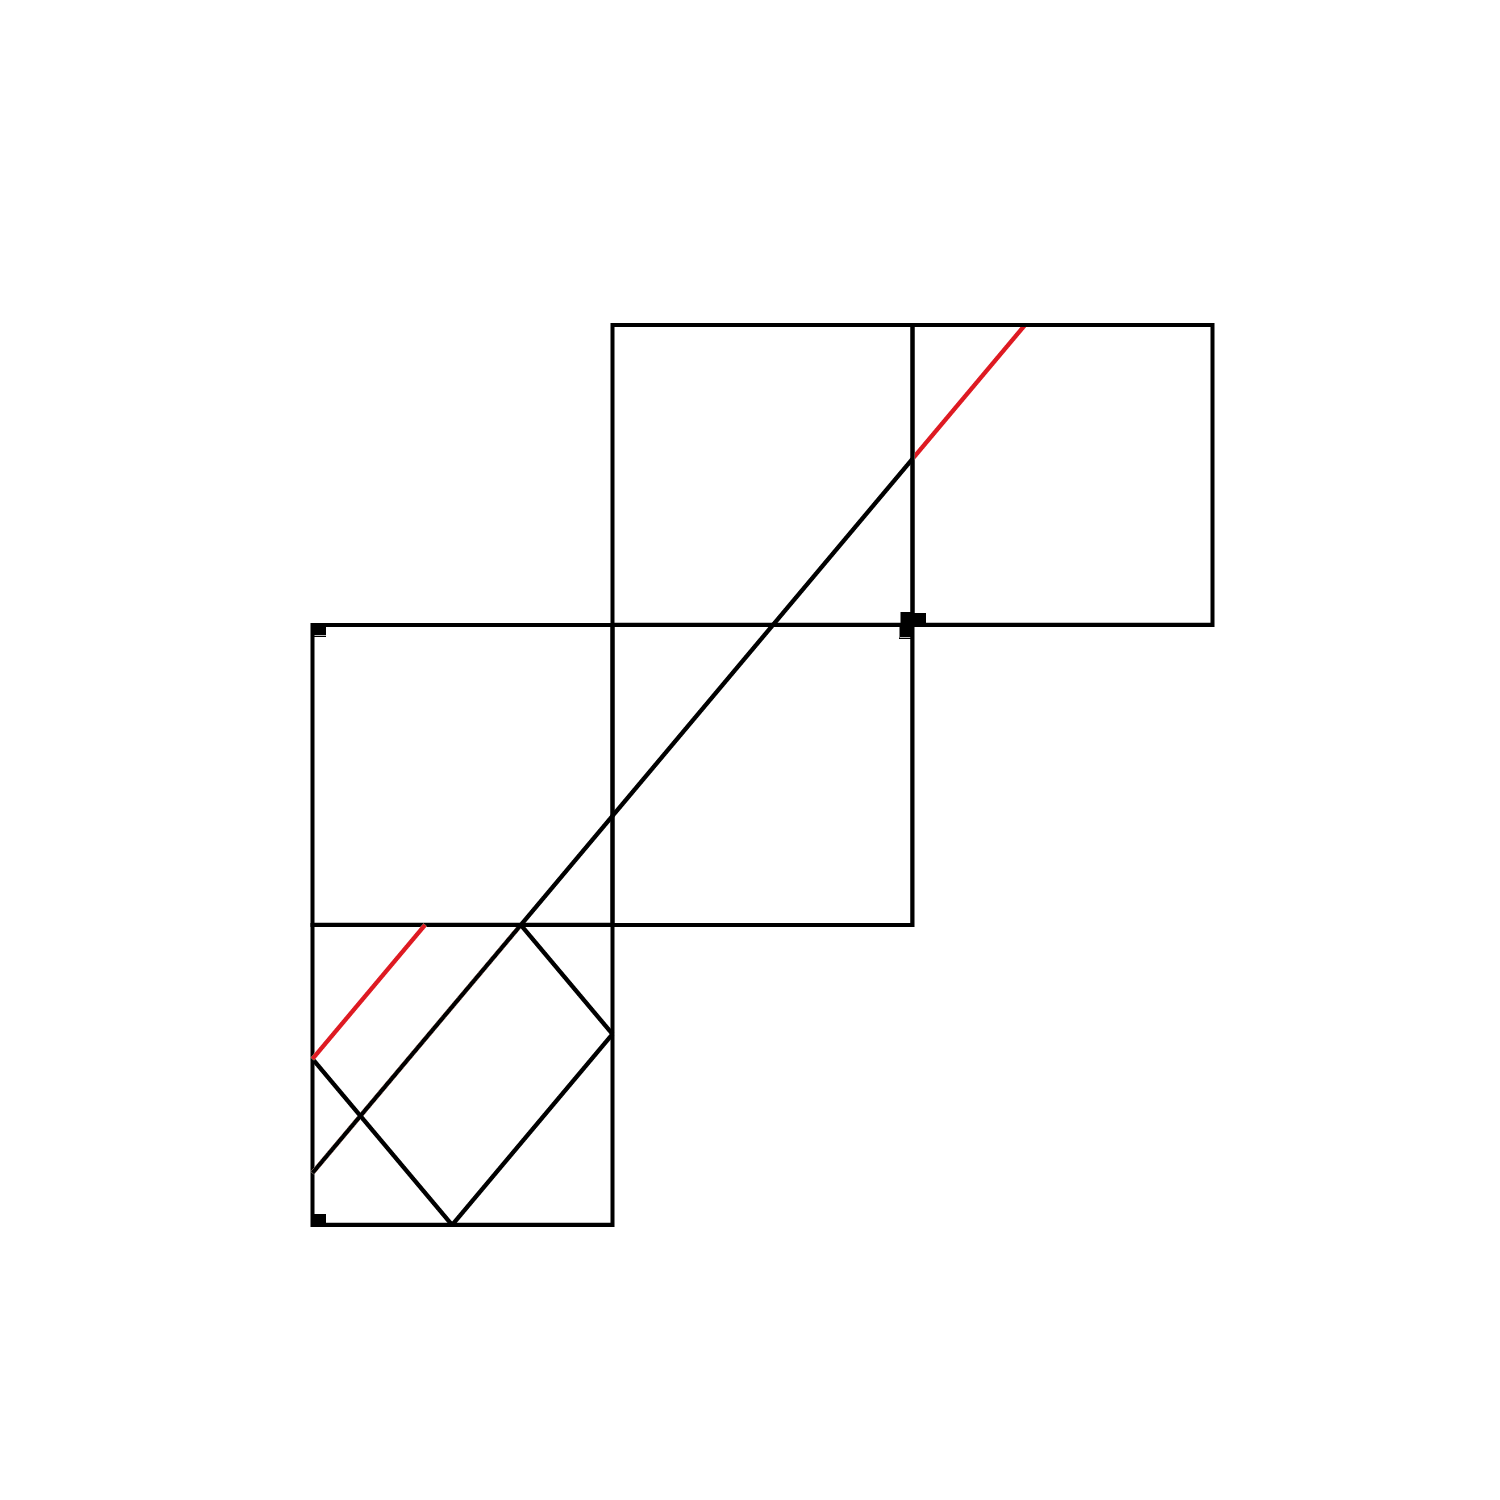
\includegraphics[width=3in]{tiling.png}
  \caption{\label{fig:tiling}Example of Tiling Billiard Tables}
\end{figure}

A couple of interesting observations can be made:

\begin{itemize}
  \item The combined trajectory $T = \{\tau(0, \kappa_1), \tau(\kappa_1, \kappa_2), \tau(\kappa_2, \kappa_3), \ldots \}$ of a ball creates a ray in the $xy$ plane.
  \item All $v$-collisions happen exactly when the combined trajectory $T$ intersects with the integer vertical lines $x = k$ where $k \in \mathrm{Z}$. The same can be said of $h$-collisions and integer horizontal lines $y = k$ for $k \in \mathrm{Z}$.
\end{itemize}

We can formalize and prove each of these observations in turn:

\begin{theorem}
  The combined trajectory $T = \{\tau(0, \kappa_1), \tau(\kappa_1, \kappa_2), \ldots\}$ of a billiard ball is a ray in the $xy$ plane under the tiling representation.
  \label{theorem:straight-line}
\end{theorem}
\begin{proof}
  We need to show that all trajectories $\tau(0, \kappa_1), \tau(\kappa_1, \kappa_2), \ldots$ which constitute the combined trajectory lie on a single line. We know that trajectories $\tau(\kappa_i, \kappa_{i+1})$ are line segments because the velocity of the billiard ball only changes during a collision. Thus, we just need to show that each trajectory $\tau(\kappa_i, \kappa_{i+1})$ lies on the same line, i.e. that $\tau(\kappa_i, \kappa_{i+2})$ is a line segment for all $i \in \mathrm{Z}$.

  We will show this by analyzing the change in trajectory at time $\kappa_i$. We know that at any time $t \in (\kappa_{i-1}, \kappa_i)$, the billiard ball will be on the line segment defined by the trajectory $\tau(\kappa_{i-1}, \kappa_i)$. This trajectory makes an angle $\theta$ with the edge $e_i$ which the billiard ball collides with at time $\kappa_i$. Moreover, we know that after colliding with $e_i$, the outgoing angle of the trajectory is equal to the incoming angle $\theta$ by our definition of collision.

The velocity is reflected about the line perpendicular to $e_i$ at the point of collision, but the angle of the trajectory $\tau(\kappa_i, \kappa_{i+1})$ makes with $e_i$ remains the same. Thus, when square $s_{i}$ is reflected about $e_i$, the resulting trajectory in $s_{i+1}$ makes an angle of $\theta$ with $e_i$. Figure \ref{fig:straight-line-angle} shows this process graphically.

\begin{figure}
  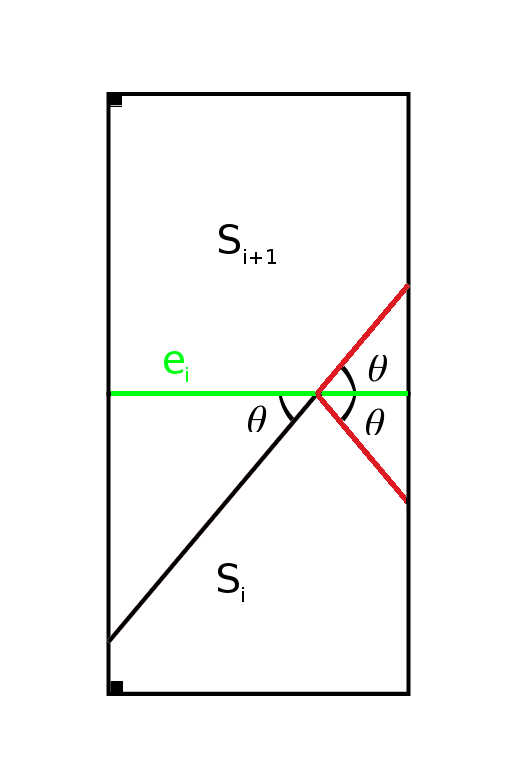
\includegraphics[height=2in]{tiling_straight_line_proof.png}
  \caption{\label{fig:straight-line-angle}Trajectories $\tau(\kappa_{i-1}, \kappa_i)$ in $s_i$ and $\tau(\kappa_{i}, \kappa_{i+1}$ $s_{i+1}$ forming a line segment}
\end{figure}

It is clear that the angles that $\tau(\kappa_{i-1}, \kappa_i)$ and $\tau(\kappa_{i}, \kappa_{i+1}$ make with $e_i$ are both $\theta$. Since both of these trajectories are already line segments, we see that the union of the two trajectories is also a line segment because both trajectories lie on the same line. Thus, we see that all trajectories $\tau(\kappa_j, \kappa_{j+1})$ for all $j \in \mathrm{Z}$ lie on the same line, which completes the proof.
\end{proof}

\begin{theorem}
  Let $t_{v, k}$ be a time when the combined trajectory $T$ intersects with some integer vertical line $x = k$ where $k \in \mathrm{Z}$. We must have $\kappa^v_k = t_{v, k}$, where $\kappa^v_k$ is the time at which the $k$th $v$-collision occurs.

  Similarly, let $t_{h, k}$ be a time when the combined trajectory $T$ intersects with some horizontal vertical line $y = k$ for $k \in \mathrm{Z}$. Then, $\kappa^h_k = t_{h, k}$.
\end{theorem}
\begin{proof}
  The proof of the first statement is exactly analogous to the proof of the second statement, so we will only prove the theorem for $\kappa^v_k = t_v$.

  Recall that in the tiling representation, whenever the billiard ball collides with an edge $e_j$, a new square $s_{j+1}$ gets reflected across $e_j$. It is clear that $e_j$, if it is a horizontal edge, lies on some integer horizontal line $y = c$ where $c \in \mathrm{Z}$. Alternatively, if $e_j$ is a vertical edge then it lies on some integer vertical line $x = c$ where $c \in \mathrm{Z}$. Thus each $\kappa_j$ corresponds to when the combined trajectory $T$ intersects with some integer vertical or integer horizontal line.

  It is also clear that the billiard ball cannot make a $v$-collision at time $t$ unless the combined trajectory $T$ intersects with an integer vertical line at time $t$ as well. Therefore, we see that $v$-collisions occur exactly when $T$ intersects with an integer vertical line.

  We know that $T$ traces a ray in the $xy$ plane by theorem \ref{theorem:straight-line}. By assumption, this ray starts in the unit square $[0,1]^2$ and has an angle between $0$ and $\pi/2$ with the horizontal. Thus, the first $v$-collision occurs when $T$ intersects $x = 1$, the second $v$-collision occurs when $T$ intersects $x = 2$, and the $k$th $v$-collision occurs when $T$ intersects $x = k$.

  However, we know that the $k$th $v$-collision occurs at time $\kappa^v_{k}$ by definition, and that the $t_{v, k}$ is the time when $T$ intersects with $x = k$. Therefore, we see that $\kappa^v_{k} = t_{v, k}$.
\end{proof}

We now see that we can represent the combined trajectory $T$ of a billiard ball as a ray in the plane. We can define the line which the ray lies on as $y = mx + y_0$, where $m$ is the slope of the line and is given by $m = \frac{\bvec{v}_y}{\bvec{v}_x}$ and $y_0$ is the $y$-intercept which can be determined by $\bvec{x}_0$ by solving for $\bvec{x}_y = m \bvec{x}_x + y_0$. This line represents the entire combined trajectory, and also determines all possible collision sequences for a particular billiard ball, since $v$-collisions happen when $x$ is an integer and $h$-collisions happen when $y$ is an integer.


\section{Simple Properties}
We will now use the tiling representation that we have developed to discover properties of collision sequences. The first simple property is that collision sequences are periodic when the initial conditions are rational numbers. Now that we can define a billiard ball as a line, instead of giving initial conditions $\bvec{x}_0$ and $\bvec{v}_0$, we can give the slope $m$ and the $y$-intercept $y_0$ of the complete trajectory's line. The formalized theorem is then:

\begin{theorem}
  \label{theorem:periodicity}
  There exists a $k \in \mathrm{N}$ such that $y_0 \equiv mk + y_0 \pmod{2}$ if and only if $m \in \mathrm{Q}$.
\end{theorem}
\begin{proof}
  Let us first show that if $m \in \mathrm{Q}$, then there exists a $k \in \mathrm{N}$ such that $y_0 \equiv mk + y_0 \pmod{2}$. We simply need to show that $0 \equiv mk \pmod{2}$ if $m \in \mathrm{Q}$. However, since we know $m \in \mathrm{Q}$, we can decompose it as follows $m = p/q$ where $p,q \in \mathrm{Z}$. Thus, we have $mk \pmod{2} \equiv \frac{pk}{q} \pmod{2}$. Now we can choose:
  \begin{eqnarray}
    k = \left\{\begin{array}{l c}
      q & \textrm{if } p \pmod{2} \equiv 0 \\
      2q & \textrm{if } p \pmod{2} \equiv 1
    \end{array}\right.
  \end{eqnarray}
  In this way, we see that $0 \equiv \frac{pk}{q} \pmod{2}$, which proves the first half of the theorem.

  Now let us show that if there exists a in $k \in \mathrm{N}$ such that $y_0 \equiv mk + y_0 \pmod[2}$, then $m \in \mathrm{Q}$. If such a $k$ exists, then we must have $0 \equiv mk \pmod{2}$, which means that $mk = 2q$ for some $q \in \mathrm{Z}$. This means $m = \frac{2q}{k}$. Now it is clear that $m \in \mathrm{Q}$ because both its numerator and denominator are integers.
\end{proof}

Theorem \ref{theorem:periodicity} shows that if $m \in \mathrm{Q}$, then the billiard ball will eventually return to it's original position $\bvec{x}_0$ with its original velocity $\bvec{v}_0$. Seeing why this is true is just a matter of using the tiling representation. We note that every second square in either the $x$ or $y$ direction is the same (because of the transitivity of reflection). Therefore, every second square will have a trajectory that exactly corresponds to the trajectory in the original square.

Thus, if $y_0 \equiv mk + y_0 \pmod{2}$, then the $y$-intercept from one of the secondary squares is the same as the $y$-intercept from the original square. Since we know that the secondary squares have the same trajectories as in the original square, we see that the trajectory will have returned to its original position (since the velocity is the same). Thus, if $y_0 \equiv mk + y_0 \pmod{2}$, then we know that the billiard ball will return to its original position with its original velocity. Theorem \ref{theorem:periodicity} also shows that if $m$ is irrational, then the billiard ball will never return to its original position and velocity.


\section{1-Dimensional Representation}
Rather than looking at an explicit representation of lines in the plane, we can gain much more insight from looking at a parametric representation. To simplify our analysis, we will choose our time parameter such that v collisions occur every $\Delta t = 1$ and h collisions occur every $\Delta t = \frac{1}{m}$. The equation for a line $y(x) = m \, x + b$ is equivalent to the following parametric system

\begin{align}\label{eq:parametric-line}
	x(t) = t + x_0\\
	y(t) = m \, t
\end{align}

Now our v and h collisions in the 2-dimensional plane can be projected onto the 1-dimensional parametric representation.

\begin{figure}[H]
  \begin{center}
    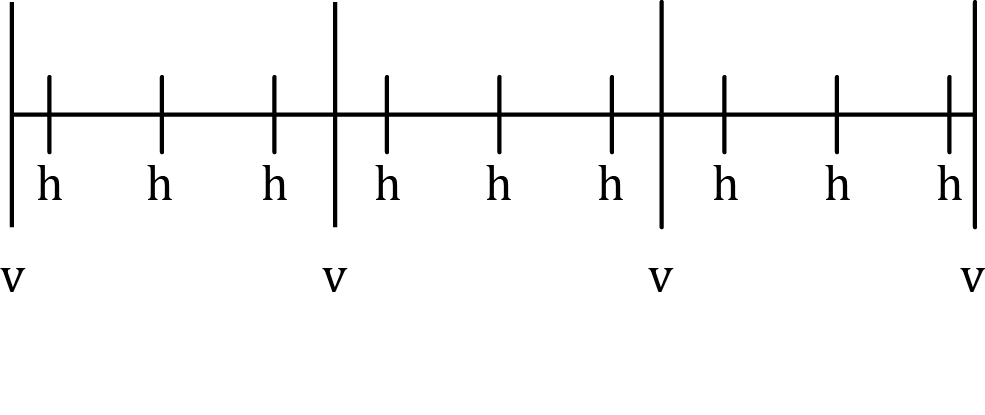
\includegraphics[keepaspectratio, width=4in]{1d_mapping_2.png}
  \end{center}
  \vspace{-.2in} % corrects bad spacing
  \caption{\label{fig:1d-projection} Projecting onto the parametric representation.}
\end{figure}

We will occasionally have to deal with some boundary conditions, and we will introduce some intermediate sequences which we will label as `augmented' and mark with a tilde. The boundary treatments are fairly pedantic and can be ignored if the reader is just interested in getting a general understanding of our solutions.

All of our theorems in this section will rely on the lengths of various patterns in the original collision sequence. We will start off by looking at the lengths of subsequences of v collisions in the collision sequence. To make this accounting simpler, we need to define an augmented collision sequence.

\begin{definition}
	\textbf{augmented collision sequence ($\tilde{\alpha}$)} which consists of the original collision sequence with one h collision added to both ends of the sequence.
\end{definition}

Now we can count lengths of v collision substrings

\begin{definition}
	\textbf{Augmented $\beta_i$:} number of v collisions between i\textsuperscript{th} and (i+1)\textsuperscript{th} h collisions in the augmented collision sequence
\end{definition}

\textbf{Still working on this part, not sure how best to deal with the boundary conditions...}

The first and last numbers in the $\beta$ sequence were artificially created by augmenting our original collision sequence. These two numbers only give us a lower bound on the number of v collisions between h collisions, so we can safely discard them if 

\begin{definition}
	\begin{align*}
		\beta_{min} \coloneqq \max_i \beta_i\\
		\beta_{max} \coloneqq \min_i \beta_i
	\end{align*}
\end{definition}

The $\beta$ sequence is much simpler to think of geometrically in terms of our parametric representation shown in Figure \ref{fig:1d-projection}. $\beta_i$ represents the number of v collision tick marks in between each h collision tick mark.

\begin{figure}[H]
  \begin{center}
    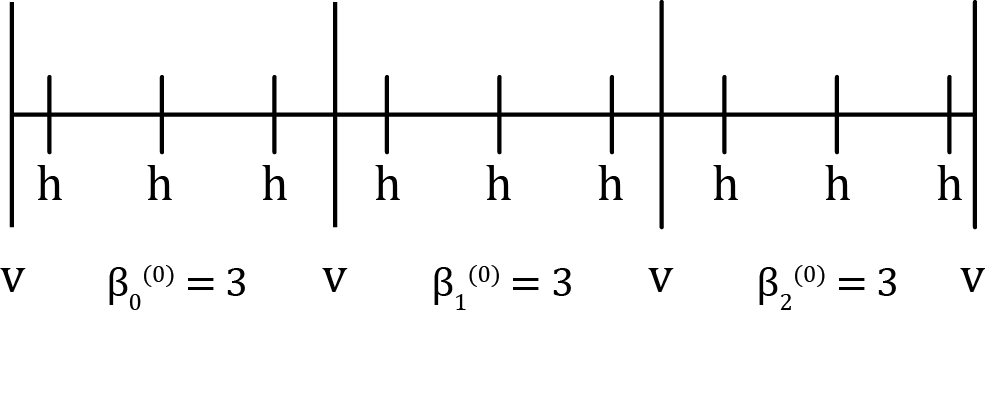
\includegraphics[keepaspectratio, width=4in]{1d_mapping_3.png}
  \end{center}
  \vspace{-.2in} % corrects bad spacing
  \caption{\label{fig:beta-sequence} The $\beta$ sequence.}
\end{figure}

\begin{lemma}
	\[
		\beta_{min} > 0
	\]
\end{lemma}

\begin{proof}
	TODO
\end{proof}

\begin{theorem}
	For every valid collision sequence, the following must be true
	
	\[
		\beta_{max} - \beta_{min} \le 1
	\]
\end{theorem}

\begin{proof}

From Equation \ref{eq:parametric-line}, v collisions occur every $\Delta t = 1$ and h collisions occur every $\Delta t = \frac{1}{m}$. Thus, the following must be true

\[
	\beta_i \in \paren{\floor{\frac{1}{m}}, \ceil{\frac{1}{m}}}
\]

For an $m$ to exist that satisfies the above constraints, all numbers in the $\beta$ sequence can only differ by 1.

\end{proof}

\begin{definition}
	\textbf{Augmented $C^{(0)}_i$:} 1 more than the number of occurrences of $\beta_{max}$ between i\textsuperscript{th} and (i+1)\textsuperscript{th} occurrence of $\beta_{min}$ in the $\beta$ sequence.
\end{definition}

\begin{theorem}
	Define 
	\begin{align*}
			\delta_i \coloneqq \begin{cases}
				x_0 \qquad &\text{if} \quad i = 0\\
				i (\ceil{\frac{1}{m}} - \frac{1}{m}) \qquad &\text{otherwise}
			\end{cases}
	\end{align*}

	Then the following is true for all valid collision sequences

	\begin{align*}
		\beta_i = \floor{\delta_i} + \beta_{max} - \floor{\delta_{i+1}}
	\end{align*}
\end{theorem}

\begin{proof}
	TODO...
\end{proof}

\section{Conclusion}
TODO

\begin{appendix}
\end{appendix}

\end{document}
